Use ifelse  for the following
\begin{enumerate}[label=\thesubsection.\arabic*, ref=\thesubsection.\theenumi]
	\item $25 \times \brak{-21} = \brak{-21}\times 25 $
	\\
	\solution 
	\lstinputlisting{codes/prog/compeq.c}
	\begin{multicols}{2}
	\item $\brak{-48}\div\brak{8} = 48 \div \brak{-8}$
	\item $\brak{-23}\times  20 = 23 \times \brak{-20}$
	\item $90 \div \brak{-45} = \brak{-90}\div 45$
	\item $ \brak{-136}\div 4=136 \div \brak{-4} $
	\item $10\times  \sbrak{6+\brak{-2}} =10\times 6+10 \times \brak{-2} $
	\item $10\times  \sbrak{6-\brak{-2}} =10\times 6-10 \times \brak{-2} $
\end{multicols}
	\item $\brak{-15}\times  \sbrak{\brak{-7}-\brak{-1}} =\brak{-15}\times\brak{-7}-\brak{-15} \times \brak{-1} $
	\item $18\times  \sbrak{\brak{7}+\brak{-3}} =18\times\brak{7}+18 \times \brak{-3} $
	\item $\brak{-21}\times  \sbrak{\brak{-4}+\brak{-6}} =\brak{-21}\times\brak{-4}+\brak{-21} \times \brak{-6} $
	\item $\brak{-15}\times  \sbrak{\brak{-7}+\brak{-1}} =\brak{-15}\times\brak{-7}+\brak{-15} \times \brak{-1} $
\end{enumerate}
\begin{enumerate}[label=\thesubsection.\arabic*, ref=\thesubsection.\theenumi,resume*]
	\item 		An angle is greater than 45\degree. Is its complementary angle greater than 45\degree or equal to 45\degree or less than 45\degree?
\end{enumerate}
	Is it possible to have a triangle with the following sides? 
\begin{enumerate}[label=\thesubsection.\arabic*, ref=\thesubsection.\theenumi,resume*]
		\begin{multicols}{2}
\item $2 cm, 3 cm, 5 cm $ 
\item $3 cm, 6 cm, 7 cm $
\item $ 6 cm, 3 cm, 2 cm$
\item $10.2 cm, 5.8 cm, 4.5 cm$?
\end{multicols}
	\end{enumerate}
	 Between which two numbers can length of the third side fall?
	The lengths of two sides of a triangle are 
\begin{enumerate}[label=\thesubsection.\arabic*, ref=\thesubsection.\theenumi,resume*]
	\begin{multicols}{2}
		\item $6 cm$ and $8 cm$.
		\item $12 cm$ and $15 cm$.
		\end{multicols}
	\end{enumerate}
Which is greater?
\begin{enumerate}[label=\thesubsection.\arabic*, ref=\thesubsection.\theenumi,resume*,itemsep=1ex]
	\begin{multicols}{2}
	\item $\frac{1}{2}$ of $\frac{3}{4}$
	or $\frac{3}{5}$ of $\frac{5}{8}$
	\item $\frac{1}{2}$ of $\frac{6}{7}$
	or $\frac{2}{3}$ of $\frac{3}{7}$
\end{multicols}
\end{enumerate}
Identify which of the following pairs of angles are complementary and which are supplementary.
\begin{enumerate}[label=\thesubsection.\arabic*, ref=\thesubsection.\theenumi,resume*]
	\begin{multicols}{4}
	\item  65\degree, 115\degree
	\item  63\degree, 27\degree 
	\item  130\degree, 50\degree 
	\item 45\degree, 45\degree 
	\item  112\degree, 68\degree 
	\item  80\degree, 10\degree
\end{multicols}
\end{enumerate}
Which of these are negative rational numbers?
\begin{enumerate}[label=\thesubsection.\arabic*, ref=\thesubsection.\theenumi,resume*,itemsep=1ex]
	\begin{multicols}{4}
	\item $\frac{-2}{3}$
	\item $\frac{5}{7}$
	\item $\frac{3}{-5}$
	\item $\frac{6}{11}$
	\item $\frac{-2}{-9}$
	\item 0
\end{multicols}
\end{enumerate}
Compare the following and fill in the blanks
\begin{enumerate}[label=\thesubsection.\arabic*, ref=\thesubsection.\theenumi,resume*,itemsep=1ex]
	\begin{multicols}{4}
		\item $\frac{-5}{7}  \dots  \frac{2}{3}$
		\item $\frac{-8}{5}  \dots  \frac{-7}{4}$
		\item ${0}  \dots  \frac{-7}{6}$
		\item $\frac{-4}{5}  \dots  \frac{-5}{7}$
		\item $\frac{1}{-3}  \dots  \frac{-1}{4}$
		\item $\frac{-7}{8}  \dots  \frac{14}{-16}$
		\item $\frac{5}{-11}  \dots  \frac{-5}{11}$
		\item $\frac{2}{3}  \dots  \frac{5}{7}$
		\item $\frac{-3}{8}  \dots  \frac{-2}{7}$
		\item $\frac{-4}{3}  \dots  \frac{-3}{2}$
		\item $\frac{-7}{21}  \dots  \frac{3}{9}$
		\item $\frac{-3}{5}  \dots  \frac{-12}{20}$
		\item $\frac{-5}{-9}  \dots  \frac{5}{-9}$
		\item $\frac{-16}{20}  \dots  \frac{20}{-25}$
		\item $\frac{8}{-5}  \dots  \frac{-24}{15}$
		\item $\frac{-2}{-3}  \dots  \frac{2}{3}$
		\item $\frac{1}{3}  \dots  \frac{-1}{9}$
		\item $\frac{4}{-9}  \dots  \frac{-16}{36}$
		\item $\frac{2}{3}  \dots  \frac{5}{2}$
		\item $\frac{-1}{4}  \dots  \frac{1}{4}$
		\item $\frac{-5}{6}  \dots  \frac{-4}{3}$
		\item $-3\frac{2}{7}  \dots  -3\frac{4}{5}$
		\item $\frac{-3}{4}  \dots  \frac{2}{-3}$
\end{multicols}
\end{enumerate}
		Write four more numbers in the following pattern
\begin{enumerate}[label=\thesubsection.\arabic*, ref=\thesubsection.\theenumi,resume*,itemsep=1ex]
	\item $\frac{-1}{3},\frac{-2}{6},\frac{-3}{9},\frac{-4}{12}$
		\\
		\solution
	\lstinputlisting{codes/prog/seq.c}
	\begin{multicols}{3}
	\item $\frac{-3}{5},\frac{-6}{10},\frac{-9}{15},\frac{-12}{20}$
	\item $\frac{-1}{4},\frac{-2}{8},\frac{-3}{12}$
	\item $\frac{-1}{6},\frac{2}{-12},\frac{3}{-18},\frac{4}{-24}$
	\item $\frac{-2}{3},\frac{2}{-3},\frac{4}{-6},\frac{6}{-9}$
\end{multicols}
		\end{enumerate}
Reduce to standard form
\begin{enumerate}[label=\thesubsection.\arabic*, ref=\thesubsection.\theenumi,resume*,itemsep=1ex]
	\begin{multicols}{4}
	\item $\frac{36}{-24}$
	\item $\frac{-3}{-15}$
	\item $\frac{-18}{45}$
	\item $\frac{-12}{18}$
	\item $\frac{-8}{6}$
	\item $\frac{25}{45}$
	\item $\frac{-44}{72}$
	\item $\frac{-8}{10}$
\end{multicols}
\end{enumerate}
Use recursion for the following
\begin{enumerate}[label=\thesubsection.\arabic*, ref=\thesubsection.\theenumi,resume*]
	\item $\brak{-1}\times\brak{-2} \times \brak{-3} \times \brak{-4}$ 
		\\
		\solution In this case,
			\begin{align}
					x(n) = -nx(n-1), x(0) = 1 
			\end{align}
			Complete the code using the above equation.
	\begin{multicols}{4}
		\item $2^6$   
		\item $11^2$
		\item $5^4$
		\item $\brak{6^2}^{4}$
		\item $\brak{2^2}^{100}$
		\item $\brak{7^{50}}^{2}$
		\item $\brak{5^3}^{7}$
		\item ${2}^{5}\times {2}^{3}$
		\item ${4}^{3}\times {4}^{2}$
		\item ${5}^{3}\times {5}^{7}\times {5}^{12}$
		\item ${2}^{8}\div{2}^{3}$
		\item ${9}^{11}\div{9}^{7}$
		\item ${7}^{13}\div{7}^{10}$
		\item ${10}^{8}\div{10}^{4}$
		\item ${20}^{15}\div{20}^{13}$
		\item $\brak{-4}^{3}$
		\item $\brak{\frac{3}{5}}^{4}$
		\item $\brak{\frac{-4}{7}}^{5}$
		\item $\brak{-4}^{100}\times \brak{-4}^{20}$
		\end{multicols}
\end{enumerate}
Use arrays for the following
\begin{enumerate}[label=\thesubsection.\arabic*, ref=\thesubsection.\theenumi,resume*]
	\item $\brak{-12}\times  \brak{-11}\times \brak{10} $
		\\
		\solution The product can be expressed as
		\begin{align}
			y = \prod_{k=0}^{2}a_k
		\end{align}
		where
		\begin{align}
			\vec{a} = \myvec{-12 \\ -11 \\ 10}
		\end{align}
	The following code implements this
	\lstinputlisting{codes/prog/prodvec.c}
	\begin{multicols}{3}
	\item $\brak{9}\times\brak{-3} \times \brak{-6}$ 
	\item $\brak{-18}\times\brak{-5} \times \brak{-4}$ 
	\item $\brak{-3}\times\brak{-6} \times \brak{-2} \times \brak{-1}$ 
\end{multicols}
\end{enumerate}
Use matrices for the following
\begin{enumerate}[label=\thesubsection.\arabic*, ref=\thesubsection.\theenumi,resume*]
\item Among two supplementary angles the measure of the larger angle is $44\degree$  more than the measure of the smaller. Find their measures.
\end{enumerate}
\begin{enumerate}[label=\thesubsection.\arabic*, ref=\thesubsection.\theenumi,resume*]
\item 
	A collection of 10 chips with different colours is given in 
\figref{fig:percent2}.
Extend the table using a C program
to include a column for the percentage of chips of each colour.
\begin{figure}[H]
  \centering
  \begin{subfigure}{0.25\textwidth}
%    
\includegraphics[width=\textwidth]{figs/percent2.jpg}
    %\documentclass{article}
%\usepackage{tikz}
%\usepackage[table]{xcolor}
%\usepackage[margin=1in]{geometry}
%
%\definecolor{lightblue}{RGB}{204, 238, 255}
%
%\begin{document}

\begin{center}
\begin{tikzpicture}
% Background
\fill[lightblue] (0,0) rectangle (4,3);

% Top row: G G G G (fully filled)
\foreach \i in {0,1,2,3} {
  \node at (\i + 0.5, 2.5) {\tikz \draw (0,0) circle (0.4cm) node {\textbf{G}};};
}

% Middle row: centered B B B (columns 0.5, 1.5, 2.5)
\foreach \i in {0,1,2} {
  \node at (\i + 0.5 + 0.5, 1.5) {\tikz \draw (0,0) circle (0.4cm) node {\textbf{B}};};
}

% Bottom row: centered R R R (columns 0.5, 1.5, 2.5)
\foreach \i in {0,1,2} {
  \node at (\i + 0.5 + 0.5, 0.5) {\tikz \draw (0,0) circle (0.4cm) node {\textbf{R}};};
}

\end{tikzpicture}
\end{center}

%\end{document}


    \caption{Chips}
  \end{subfigure}
  \hfill
\begin{subfigure}{0.4\textwidth}
%    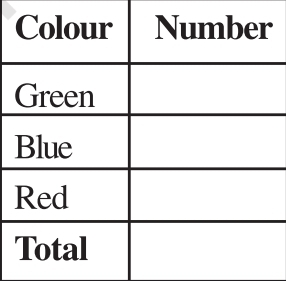
\includegraphics[width=\textwidth]{figs/percent3.jpg}
	  %%%%%%%%%%%%%%%%%%%%%%%%%%%%%%%%%%%%%%%%%%%%%%%%%%%%%%%%%%%%%%%%%%%%%%
%%                                                                  %%
%%  This is the header of a LaTeX2e file exported from Gnumeric.    %%
%%                                                                  %%
%%  This file can be compiled as it stands or included in another   %%
%%  LaTeX document. The table is based on the longtable package so  %%
%%  the longtable options (headers, footers...) can be set in the   %%
%%  preamble section below (see PRAMBLE).                           %%
%%                                                                  %%
%%  To include the file in another, the following two lines must be %%
%%  in the including file:                                          %%
%%        \def\inputGnumericTable{}                                 %%
%%  at the beginning of the file and:                               %%
%%        \input{name-of-this-file.tex}                             %%
%%  where the table is to be placed. Note also that the including   %%
%%  file must use the following packages for the table to be        %%
%%  rendered correctly:                                             %%
%%    \usepackage[latin1]{inputenc}                                 %%
%%    \usepackage{color}                                            %%
%%    \usepackage{array}                                            %%
%%    \usepackage{longtable}                                        %%
%%    \usepackage{calc}                                             %%
%%    \usepackage{multirow}                                         %%
%%    \usepackage{hhline}                                           %%
%%    \usepackage{ifthen}                                           %%
%%  optionally (for landscape tables embedded in another document): %%
%%    \usepackage{lscape}                                           %%
%%                                                                  %%
%%%%%%%%%%%%%%%%%%%%%%%%%%%%%%%%%%%%%%%%%%%%%%%%%%%%%%%%%%%%%%%%%%%%%%



%%  This section checks if we are begin input into another file or  %%
%%  the file will be compiled alone. First use a macro taken from   %%
%%  the TeXbook ex 7.7 (suggestion of Han-Wen Nienhuys).            %%
\def\ifundefined#1{\expandafter\ifx\csname#1\endcsname\relax}


%%  Check for the \def token for inputed files. If it is not        %%
%%  defined, the file will be processed as a standalone and the     %%
%%  preamble will be used.                                          %%
\ifundefined{inputGnumericTable}

%%  We must be able to close or not the document at the end.        %%
	\def\gnumericTableEnd{\end{document}}


%%%%%%%%%%%%%%%%%%%%%%%%%%%%%%%%%%%%%%%%%%%%%%%%%%%%%%%%%%%%%%%%%%%%%%
%%                                                                  %%
%%  This is the PREAMBLE. Change these values to get the right      %%
%%  paper size and other niceties.                                  %%
%%                                                                  %%
%%%%%%%%%%%%%%%%%%%%%%%%%%%%%%%%%%%%%%%%%%%%%%%%%%%%%%%%%%%%%%%%%%%%%%

	\documentclass[12pt%
			  ,landscape%
                    ]{report}
       \usepackage[latin1]{inputenc}
       \usepackage{fullpage}
       \usepackage{color}
       \usepackage{array}
       \usepackage{longtable}
       \usepackage{calc}
       \usepackage{multirow}
       \usepackage{hhline}
       \usepackage{ifthen}

	\begin{document}


%%  End of the preamble for the standalone. The next section is for %%
%%  documents which are included into other LaTeX2e files.          %%
\else

%%  We are not a stand alone document. For a regular table, we will %%
%%  have no preamble and only define the closing to mean nothing.   %%
    \def\gnumericTableEnd{}

%%  If we want landscape mode in an embedded document, comment out  %%
%%  the line above and uncomment the two below. The table will      %%
%%  begin on a new page and run in landscape mode.                  %%
%       \def\gnumericTableEnd{\end{landscape}}
%       \begin{landscape}


%%  End of the else clause for this file being \input.              %%
\fi

%%%%%%%%%%%%%%%%%%%%%%%%%%%%%%%%%%%%%%%%%%%%%%%%%%%%%%%%%%%%%%%%%%%%%%
%%                                                                  %%
%%  The rest is the gnumeric table, except for the closing          %%
%%  statement. Changes below will alter the table's appearance.     %%
%%                                                                  %%
%%%%%%%%%%%%%%%%%%%%%%%%%%%%%%%%%%%%%%%%%%%%%%%%%%%%%%%%%%%%%%%%%%%%%%

\providecommand{\gnumericmathit}[1]{#1} 
%%  Uncomment the next line if you would like your numbers to be in %%
%%  italics if they are italizised in the gnumeric table.           %%
%\renewcommand{\gnumericmathit}[1]{\mathit{#1}}
\providecommand{\gnumericPB}[1]%
{\let\gnumericTemp=\\#1\let\\=\gnumericTemp\hspace{0pt}}
 \ifundefined{gnumericTableWidthDefined}
        \newlength{\gnumericTableWidth}
        \newlength{\gnumericTableWidthComplete}
        \newlength{\gnumericMultiRowLength}
        \global\def\gnumericTableWidthDefined{}
 \fi
%% The following setting protects this code from babel shorthands.  %%
 \ifthenelse{\isundefined{\languageshorthands}}{}{\languageshorthands{english}}
%%  The default table format retains the relative column widths of  %%
%%  gnumeric. They can easily be changed to c, r or l. In that case %%
%%  you may want to comment out the next line and uncomment the one %%
%%  thereafter                                                      %%
\providecommand\gnumbox{\makebox[0pt]}
%%\providecommand\gnumbox[1][]{\makebox}

%% to adjust positions in multirow situations                       %%
\setlength{\bigstrutjot}{\jot}
\setlength{\extrarowheight}{\doublerulesep}

%%  The \setlongtables command keeps column widths the same across  %%
%%  pages. Simply comment out next line for varying column widths.  %%
\setlongtables

\setlength\gnumericTableWidth{%
	41pt+%
	45pt+%
0pt}
\def\gumericNumCols{2}
\setlength\gnumericTableWidthComplete{\gnumericTableWidth+%
         \tabcolsep*\gumericNumCols*2+\arrayrulewidth*\gumericNumCols}
\ifthenelse{\lengthtest{\gnumericTableWidthComplete > \linewidth}}%
         {\def\gnumericScale{1*\ratio{\linewidth-%
                        \tabcolsep*\gumericNumCols*2-%
                        \arrayrulewidth*\gumericNumCols}%
{\gnumericTableWidth}}}%
{\def\gnumericScale{1}}

%%%%%%%%%%%%%%%%%%%%%%%%%%%%%%%%%%%%%%%%%%%%%%%%%%%%%%%%%%%%%%%%%%%%%%
%%                                                                  %%
%% The following are the widths of the various columns. We are      %%
%% defining them here because then they are easier to change.       %%
%% Depending on the cell formats we may use them more than once.    %%
%%                                                                  %%
%%%%%%%%%%%%%%%%%%%%%%%%%%%%%%%%%%%%%%%%%%%%%%%%%%%%%%%%%%%%%%%%%%%%%%

\ifthenelse{\isundefined{\gnumericColA}}{\newlength{\gnumericColA}}{}\settowidth{\gnumericColA}{\begin{tabular}{@{}p{41pt*\gnumericScale}@{}}x\end{tabular}}
\ifthenelse{\isundefined{\gnumericColB}}{\newlength{\gnumericColB}}{}\settowidth{\gnumericColB}{\begin{tabular}{@{}p{45pt*\gnumericScale}@{}}x\end{tabular}}

\begin{longtable}[c]{%
	b{\gnumericColA}%
	b{\gnumericColB}%
	}

%%%%%%%%%%%%%%%%%%%%%%%%%%%%%%%%%%%%%%%%%%%%%%%%%%%%%%%%%%%%%%%%%%%%%%
%%  The longtable options. (Caption, headers... see Goosens, p.124) %%
%	\caption{The Table Caption.}             \\	%
% \hline	% Across the top of the table.
%%  The rest of these options are table rows which are placed on    %%
%%  the first, last or every page. Use \multicolumn if you want.    %%

%%  Header for the first page.                                      %%
%	\multicolumn{2}{c}{The First Header} \\ \hline 
%	\multicolumn{1}{c}{colTag}	%Column 1
%	&\multicolumn{1}{c}{colTag}	\\ \hline %Last column
%	\endfirsthead

%%  The running header definition.                                  %%
%	\hline
%	\multicolumn{2}{l}{\ldots\small\slshape continued} \\ \hline
%	\multicolumn{1}{c}{colTag}	%Column 1
%	&\multicolumn{1}{c}{colTag}	\\ \hline %Last column
%	\endhead

%%  The running footer definition.                                  %%
%	\hline
%	\multicolumn{2}{r}{\small\slshape continued\ldots} \\
%	\endfoot

%%  The ending footer definition.                                   %%
%	\multicolumn{2}{c}{That's all folks} \\ \hline 
%	\endlastfoot
%%%%%%%%%%%%%%%%%%%%%%%%%%%%%%%%%%%%%%%%%%%%%%%%%%%%%%%%%%%%%%%%%%%%%%

\hhline{|-|-}
	 \multicolumn{1}{|p{\gnumericColA}|}%
	{\gnumericPB{\centering}\textbf{Colour}}
	&\multicolumn{1}{p{\gnumericColB}|}%
	{\gnumericPB{\centering}\textbf{Number}}
\\
\hhline{|--|}
	 \multicolumn{1}{|p{\gnumericColA}|}%
	{\gnumericPB{\centering}Green}
	&\multicolumn{1}{p{\gnumericColB}|}%
	{}
\\
\hhline{|--|}
	 \multicolumn{1}{|p{\gnumericColA}|}%
	{\gnumericPB{\centering}\gnumbox{Blue}}
	&\multicolumn{1}{p{\gnumericColB}|}%
	{}
\\
\hhline{|--|}
	 \multicolumn{1}{|p{\gnumericColA}|}%
	{\gnumericPB{\centering}\gnumbox{Red}}
	&\multicolumn{1}{p{\gnumericColB}|}%
	{}
\\
\hhline{|--|}
	 \multicolumn{1}{|p{\gnumericColA}|}%
	{\gnumericPB{\centering}\gnumbox{Total}}
	&\multicolumn{1}{p{\gnumericColB}|}%
	{}
\\
\hhline{|-|-|}
\end{longtable}

\ifthenelse{\isundefined{\languageshorthands}}{}{\languageshorthands{\languagename}}
\gnumericTableEnd

    \caption{Table}
  \end{subfigure}
  \caption{}
  \label{fig:percent2}
\end{figure}
	\solution 
	\lstinputlisting{codes/prog/percent.c}
\end{enumerate}
